\section{System Test Report}
In dit hoofstuk worden de testresultaten behandeld, de testplannen hiervoor staan in het vorige hoofdstuk genaamd System test plan.

\subsection{MQTT communicatie}
Voor het testen van de communicatie MQTT, zijn aparte test files geschreven. De messages worden gevormd in de ene test file genaamd test\_publish.py. Deze kunnen vervolgens succesvol worden uitgelezen in test\_recieve.py.

\subsection{Camera object tracking}
De camera kan in een live beeld de drone onderscheiden ende locatie van deze drone aangeven. Vervolgens worden deze pixel coordinaten omgevormd naar grid coordinaten die doorgestuurd worden. In de afbeelding is te zien hoe de drone wordt onderscheiden van zijn omgeving en coordinaten aan hem worden toegepast.
\begin{center}
    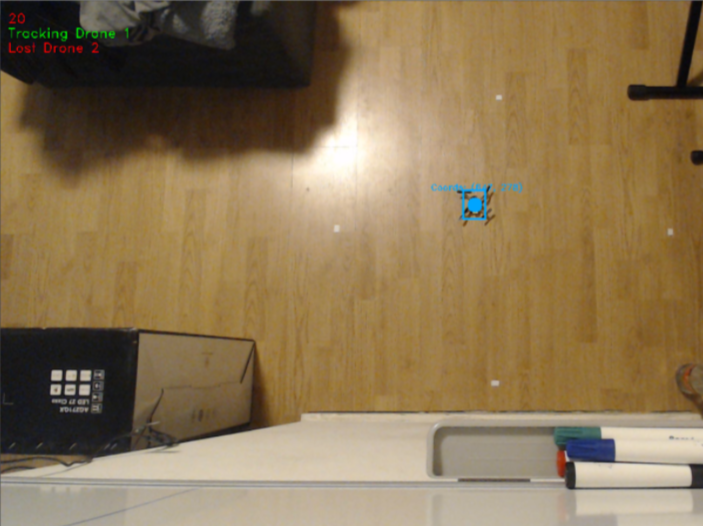
\includegraphics[scale=0.5]{trackedDrone.png}
\end{center}



\subsection{Drone Foodsearch}
De crazyflie heeft soms problemen met opstijgen door een lage batterij, maar zolang de batterij minstens 25 procent batterij heeft is er niks aan de hand en vliegt de drone, via kleine, snelle stappen, naar de voedselbron volgens de route die pathfinding geplanned heeft. Zodra de drone geland is op de voedselbron stijgt hij weer op om terug te keren naar de korf, als geariveerd begint hij met dansen door 360 graden links en dan 360 graden rechts te draaien. Na het dansen land hij in de korf, mogelijk is hij een beetje verplaatst door het dansen, maar niet zoveel dat hij buiten de korf zou komen.
Deze test is ook te zien in filmpje dat hoort bij de opleverset.

\subsection{Drone Foodget}
Het gedrag van de drone is voor het eerste vlieggedeelte hetzelfde als bij de Foodsearch. Echter zodra hij bij de korf arriveert land hij en zolang de voedselbron nog niet leeg is stijgt hij weer op om het te herhalen.
Dit gedeelte van de test werkt, maar de collision avoidance werkt op het moment van het inleveren van dit rapport helaas nog niet, dit zal in de toekomst nog gedaan worden.

\subsection{Crazyflie weergeven in simulatie}
De informatie voor de locatie van de Crazyflie wordt doorgegeven door middel van MQTT messages. Met de binnengekomen berichten wordt het verschil in thuis en verplaasting uitgerekend zodat de beweging in de simulatie vloeiend is. Deze test is te zien in de bijgeleverde video in de opleveset.
\begin{center}
    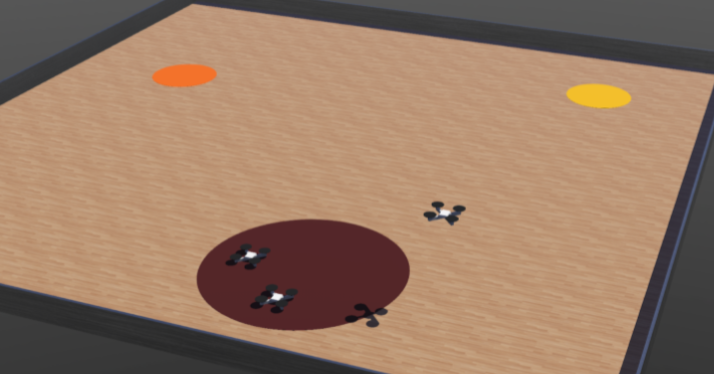
\includegraphics[scale=0.5]{simdrone.png}
\end{center}